\section{Appendix}

\subsection*{Appendix A: Detailed Charts}\label{sec:detailed_charts}

\begin{figure}[H]
    \centering
    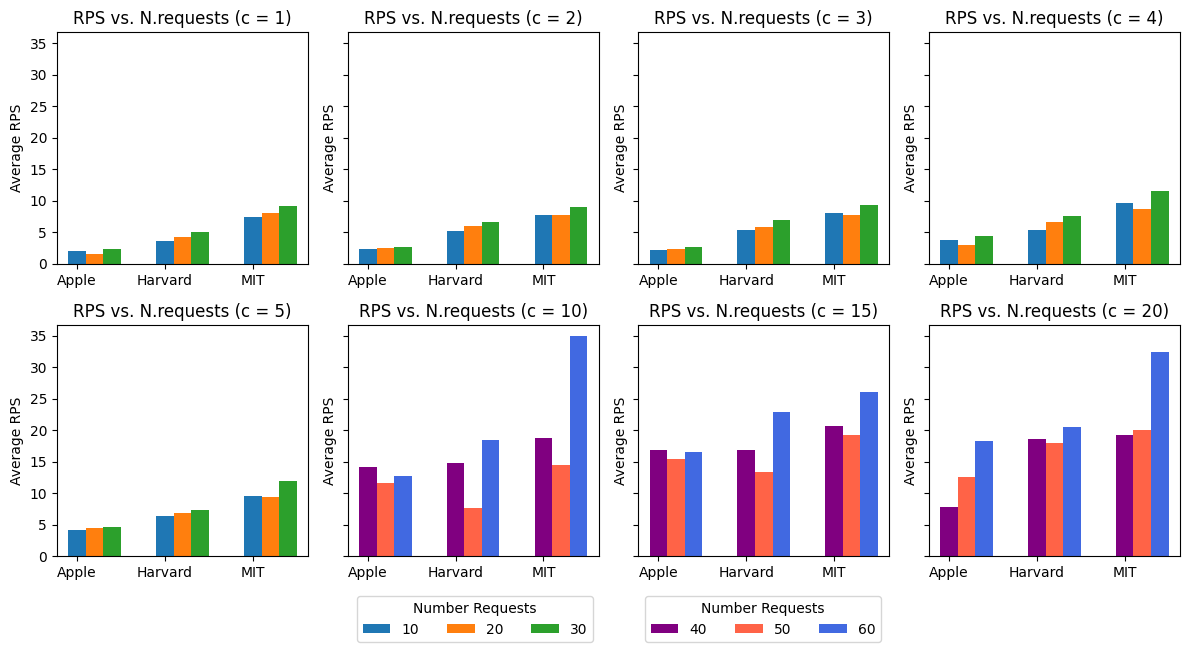
\includegraphics[width=0.90\textwidth]{4_detailed.png}
    \caption{\small Detailed analysis RPS vs Number of requests and Concurrency level}
    \label{fig:4_detailed}
\end{figure}

\begin{figure}[H]
    \centering
    \includegraphics[width=0.90\textwidth]{5_RPS_detailed.png}
    \caption{\small RPS and Warm-up time for different concurrency levels}
    \label{fig:5_RPS_detailed}
\end{figure}

\begin{figure}[H]
    \centering
    \includegraphics[width=0.90\textwidth]{5_TPR_detailed.png}
    \caption{\small TPR and Warm-up time for different concurrency levels}
    \label{fig:5_TPR_detailed}
\end{figure}

\begin{figure}[H]
    \centering
    \includegraphics[width=0.90\textwidth]{5_SD_detailed.png}
    \caption{\small SD and Warm-up time for different concurrency levels}
    \label{fig:5_SD_detailed}
\end{figure}


\subsection*{Appendix B: Scripts}\label{sec:scripts}

\begin{figure}[H]
    \centering
    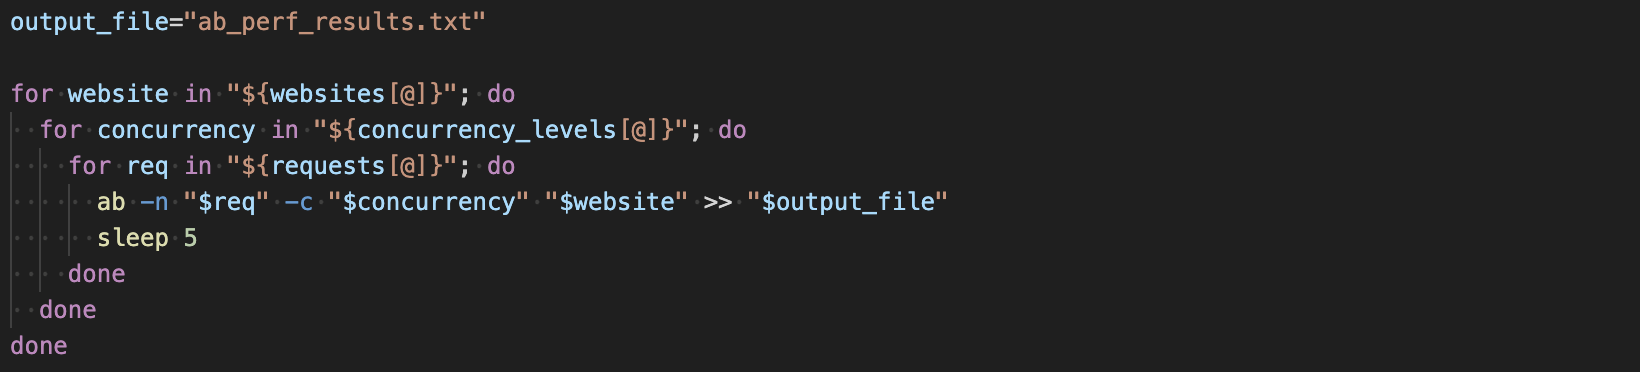
\includegraphics[width=0.90\textwidth]{4_ab_perf_script.png}
    \caption{\small Bash script for ab experiments}
    \label{fig:4_ab_perf_script}
\end{figure}

\begin{figure}[H]
    \centering
    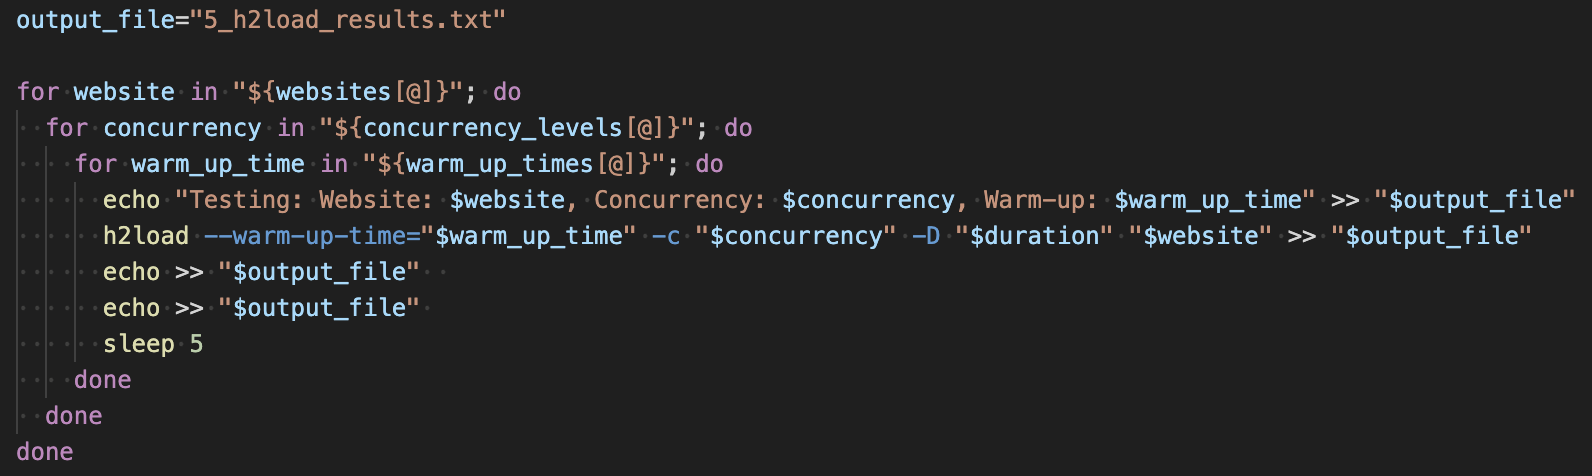
\includegraphics[width=0.90\textwidth]{5_h2load_script.png}
    \caption{\small Bash script for h2load experiments}
    \label{fig:5_h2load_script}
\end{figure}
